\documentclass{article}

\include{stddefs}
\include{imodefs}

\chapterno{3}

\begin{document}

\chapter{Matrices}\label{Chapter:Matrices}


Handling linear equations and keeping track of the unknowns can be a pain. At
a certain point one needs to simplify the notation. This is done introducing
matrices. 

For example, the system of equations
\begin{equation}\label{equ2l}
\begin{matrix}
&&  &2y &+ &4z &= &-2\\
&3x &+ &2y &+ &7z &= &4
\end{matrix}
\end{equation}
can be represented by the rectangular array (matrix)
\begin{equation}\label{matrix1} 
\begin{pmatrix}
0 & 2 & 4 & -2\\
3 & 2 & 7 & 4
\end{pmatrix}
\end{equation}
of numbers. Many of the operations we do to solve linear equations might as well be done on this array forgetting
about the unknowns.

\section{Matrices}

\subsection{Definitions}
A rectangular array of numbers is called a \index{matrix}\emph{matrix}. A matrix with $m$ \emph{rows} and $n$ 
\emph{columns} is called an $m\times n$ ($m$ by $n$) matrix. 
The notation for an $m\times n$ matrix $A$ is
\begin{equation}\label{matr}
A =  
\begin{pmatrix}
a_{11} & \cdots &a_{1j}& \cdots& a_{1 n} \\
\vdots & \ddots &\vdots & \ddots & \vdots\\
a_{i1} & \cdots &a_{ij}& \cdots& a_{i n} \\
\vdots & \ddots &\vdots & \ddots & \vdots\\
a_{m1} & \cdots &a_{mj}& \cdots& a_{m n}
\end{pmatrix},
\end{equation}
where $A_{ij} = a_{i j}$ denotes the number or \emph{entry} in the  $i$-th row and $j$-th column. If the matrix in \eqref{matrix1}
is denoted $A$, then it has $2$ rows and $4$ columns with $A_{14} = -2$.

Two matrices are equal if they have the same number of rows and columns and their entries are
identical.
 
Sage is built on top of python and has access to all its libraries. A
very useful (and famous) library for handling matrices is \texttt{numpy}. Here is how
the matrix in \eqref{matrix1} is entered in \texttt{numpy}.

\begin{sage}
import numpy as np
  
m = np.matrix( [[0, 2, 4, -2], [3, 2, 7, 4]] )
print(m)
\end{sage}


\begin{enumerate}

\item
  A matrix whose entries are all $0$ is called a zero matrix. It is denoted simply by $0$, when
  it is clear from the context what its numbers of rows and columns are.
  
\item
  A matrix is called  \emph{quadratic}\index{quadratic matrix} if it has an equal number of rows and columns.
  The first two matrices below are quadratic, whereas the third is not.
$$
\begin{pmatrix} 1 \end{pmatrix}, \qquad
\begin{pmatrix} 1 & 2 & 3\\ 4 & 5 & 6\\ 7 & 8 & 9\end{pmatrix}, \qquad
\begin{pmatrix} 0 & 1 & 0\\ 1 & 0 & 1\end{pmatrix}.
$$
\item 
\label{diagonalmat}
The \emph{diagonal} in a matrix is defined as the entries in the matrix with the same row- and column indices.
Below we have a $3\times 4$ matrix with the diagonal elements marked
$$
\begin{pmatrix}
\color{red}{1} & 3 & 0 & 1\\
3 & \color{red}{2} & 1 & 5\\
1 & 0 & \color{red}{3} & 6
\end{pmatrix}.
$$
A matrix is called a \index{diagonal matrix}\emph{diagonal matrix}, if all its entries outside the
diagonal are $=0$. Below is an example of a square diagonal matrix
$$
\begin{pmatrix}
1 & 0 & 0\\
0 & 2 & 0\\
0 & 0 & 3
\end{pmatrix}.
$$
\item
A matrix is called a \index{row vector}\emph{row vector} if it has only one row. For example,
$$
\begin{pmatrix}
1 & 2 & 3
\end{pmatrix}
$$
is a row vector with three columns.
\item
A matrix is called a \index{column vector}\emph{column vector} if it has only one column.
For example, 
$$
\begin{pmatrix}
1\\ 2 \\ 3
\end{pmatrix}
$$
is a column vector with three rows.
\item
  The rows in a matrix are called the  \emph{row vectors} of the matrix.
The $i$-th row in a matrix $A$ is denoted $A_i$.
The matrix $A$ in \eqref{matrix1} contains the row vectors
$$
A_1 = \begin{pmatrix}
0 & 2 & 4 & -2
\end{pmatrix}
\qquad\text{and}\qquad
A_2 = \begin{pmatrix}
3 & 2 & 7 & 4
\end{pmatrix}.
$$
\item
  The columns in a matrix are called the \emph{column vectors} of the matrix.
The $j$-th column in a matrix $A$ is denoted \footnote{$A^j$}{Not to be confused with powers of the matrix $A$ introduced later.}.
The matrix $A$ in \eqref{matrix1} contains the column vectors
$$
A^1 = \begin{pmatrix}
0 \\ 3
\end{pmatrix},\quad
A^2 =\begin{pmatrix}
2 \\ 2
\end{pmatrix},\quad
A^3 =\begin{pmatrix}
4 \\ 7
\end{pmatrix}\quad\text{and}\quad
A^4 = \begin{pmatrix}
-2 \\ 4
\end{pmatrix}.
$$
 
\item
  A row- or column vector is referred to as a \index{vector}\emph{vector}.
\item
  Even though we have used the notation $\RR^n$ for the $n$-th cartesian product of $\RR$, we
  will use $\RR^n$ henceforth to denote the set of column vectors with $n$ rows (entries). This
  definition is almost identical with the previous one, except that the tuple is formatted as
  a column vector.

  Illustrated by an example, 
  $$
  \begin{pmatrix} 1 \\ 2 \\ 3 \end{pmatrix} \in \RR^3\qquad\text{instead of}\qquad (1, 2, 3)\in \RR^3.
  $$
\end{enumerate}



\section{Linear maps}\label{sectionLM}

In the first chapter we encountered a miniature version of a neural
network. Neural networks are generally incredibly complicated functions
from $\RR^n$ to $\RR^m$. The function $f:\RR^2\rightarrow \RR^2$
given by
$$
f\begin{pmatrix}
  x \\ y
\end{pmatrix} =
\begin{pmatrix}
  x^7 y + \cos(x y) e^{x^2 + y^2 -1}\\
  2 x y^2 - \sin(x + y) (x^3 + y^3)
\end{pmatrix},
$$
even though it looks complicated, is simple in comparison.

You probably agree that the function $g:\RR^2\rightarrow \RR^2$ given by
$$
g\begin{pmatrix}
  x \\ y
\end{pmatrix} =
\begin{pmatrix}
  2 x + 3 y\\
  3 x - 2 y
\end{pmatrix}
$$
is even simpler. This function (or map) is an example of a linear map.
In general, a \emph{linear map}
$f: \RR^n\rightarrow \RR^m$ has the form
$$
f\begin{pmatrix}
  x_1 \\ \vdots \\ x_n
\end{pmatrix} =
\begin{pmatrix}
  a_{11} x_1 + \cdots + a_{1 n} x_n\\
  \vdots \\
  a_{m1} x_1 + \cdots + a_{m n} x_n
\end{pmatrix},
$$
where $a_{11}, \dots, a_{mn}$ are $m n$ real numbers.

Using matrices we will use the notation
$$
\begin{pmatrix}
a_{11} & \cdots & a_{1n}\\
\vdots & \ddots & \vdots\\
a_{m1} & \cdots & a_{mn}
\end{pmatrix}
\begin{pmatrix} x_1 \\ \vdots \\ x_n\end{pmatrix} =
\begin{pmatrix}
  a_{11} x_1 + \cdots + a_{1 n} x_n\\
  \vdots \\
  a_{m1} x_1 + \cdots + a_{m n} x_n
\end{pmatrix}.
$$


In this way, we can write the map $f$ as
$$
f(v) = A v,
$$
where $A$ is the $m\times n$ matrix
$$
\begin{pmatrix}
a_{11} & \cdots & a_{1n}\\
\vdots & \ddots & \vdots\\
a_{m1} & \cdots & a_{mn}
\end{pmatrix}
$$
and $v$ is the vector
$$
\begin{pmatrix} x_1 \\ \vdots \\ x_n\end{pmatrix}
$$
in $\RR^n$.

Basically a linear map is a system of linear equations without the right hand side (including $=$).
In fact, we may write the system of linear equations in \eqref{equ2l} as
$$
\begin{pmatrix}
0 & 2 & 4\\
3 & 2 & 7
\end{pmatrix}
\begin{pmatrix}
  x \\ y \\ z
\end{pmatrix}
=
\begin{pmatrix}
  -2 \\ 4
\end{pmatrix}.
$$
\beginshex
Let $f: \RR^2\rightarrow \RR^2$ be the linear map given by the $2\times 2$ matrix
$$
\begin{pmatrix}
  1 & 2\\
  3 & 4
\end{pmatrix}.
$$
Does there exist $u\in \RR^2$, such that
$$
f(u) = \begin{pmatrix} 3 \\ 7 \end{pmatrix}?
$$
Quite generally, can we find $u\in \RR^2$, such that
$$
f(u) = \begin{pmatrix} b_1 \\ b_2 \end{pmatrix}?
$$
for arbitrary $b_1, b_2\in \RR$?
\endshex

\beginshex
Suppose you know that $f: \RR^n\rightarrow \RR^m$ is a linear map and
that you have a black box giving you output $f(v)\in \RR^m$ if you
supply the input $v\in \RR^n$. How would you find
the matrix defining $f$?
\endshex


\section{Matrix multiplication}

Suppose we are given two linear maps $f: \RR^2\rightarrow \RR^2$ and
$g:\RR^2\rightarrow \RR^2$. Then it turns out that the composition
$f\circ g: \RR^2\rightarrow \RR^2$ is also a linear map. A word of advice:
the computations below look large and intimidating. They are not. It
is important that you carry them out on your own. Do not look and copy or tell
yourself that it looks okay. Do the computations yourself and ask me
or fellow students if you get stuck.

Let us look at an example. Suppose that
$$
g\begin{pmatrix} x\\ y \end{pmatrix} =
\begin{pmatrix}
  2 & 3 \\
  -1 & -2
\end{pmatrix}
\begin{pmatrix}
  x \\ y
\end{pmatrix}\qquad
\text{and}
\qquad
f\begin{pmatrix} u\\ v \end{pmatrix} =
\begin{pmatrix}
  1 & 2 \\
  1 & -2
\end{pmatrix}
\begin{pmatrix}
  u \\ v
\end{pmatrix}.
$$
Then
\begin{align*}
(f\circ g)\begin{pmatrix} x\\ y \end{pmatrix} &=
f\left(g\begin{pmatrix} x\\ y \end{pmatrix}\right) =
f\left(\begin{pmatrix}
  2 & 3 \\
  -1 & -2
\end{pmatrix}
\begin{pmatrix}
  x \\ y
\end{pmatrix}\right)
=
\begin{pmatrix}
  1 & 2 \\
  1 & -2
\end{pmatrix}
      \left(
\begin{pmatrix}
  2 & 3 \\
  -1 & -2
\end{pmatrix}
\begin{pmatrix}
  x \\ y
\end{pmatrix}
  \right)\\
  \\
  &= 
\begin{pmatrix}
  1 & 2 \\
  1 & -2
\end{pmatrix}
\begin{pmatrix}
  2 x + 3 y\\
  -x - 2y
\end{pmatrix} =
  \begin{pmatrix}
    - y \\
    4 x + 7 y
  \end{pmatrix}
  =
  \begin{pmatrix}
    0 & -1\\
    4 & 7
  \end{pmatrix}
  \begin{pmatrix}
    x \\ y
  \end{pmatrix}.
\end{align*}

In terms of the matrices of the linear maps, we write this as
\begin{equation}\label{moperation}
\begin{pmatrix}
1 & 2\\
1 & -2
\end{pmatrix}
\begin{pmatrix}
2 & 3\\
-1 & -2
\end{pmatrix}
=
\begin{pmatrix}
0 & -1\\
4 & 7
\end{pmatrix}
\end{equation}

There is nothing special about the numbers in this example. We might as well
do the computation in general: suppose that

$$
g\begin{pmatrix} x\\ y \end{pmatrix} =
\begin{pmatrix}
  b_{11} & b_{12} \\
  b_{21} & b_{22}
\end{pmatrix}
\begin{pmatrix}
  x \\ y
\end{pmatrix}\qquad
\text{and}
\qquad
f\begin{pmatrix} u\\ v \end{pmatrix} =
\begin{pmatrix}
  a_{11} & a_{12} \\
  a_{21} & a_{22}
\end{pmatrix}
\begin{pmatrix}
  u \\ v
\end{pmatrix}.
$$
Then
\begin{align*}
(f\circ g)\begin{pmatrix} x\\ y \end{pmatrix} &=
f\left(g\begin{pmatrix} x\\ y \end{pmatrix}\right) =
f\left(\begin{pmatrix}
  b_{11} & b_{12} \\
  b_{21} & b_{22}
\end{pmatrix}
\begin{pmatrix}
  x \\ y
\end{pmatrix}\right)
=
\begin{pmatrix}
  a_{11} & a_{12} \\
  a_{21} & a_{22}
\end{pmatrix}
      \left(
\begin{pmatrix}
  b_{11} & b_{12} \\
  b_{21} & b_{22}
\end{pmatrix}
\begin{pmatrix}
  x \\ y
\end{pmatrix}
  \right)\\
  \\
  &= 
\begin{pmatrix}
  a_{11} & a_{12} \\
  a_{21} & a_{22}
\end{pmatrix}
\begin{pmatrix}
  b_{11} x + b_{12} y\\
  b_{21} x + b_{22} y
\end{pmatrix} =
  \begin{pmatrix}
a_{11} (b_{11} x + b_{12} y) + a_{12} (b_{21} x + b_{22} y)\\
a_{21} (b_{11} x + b_{12} y) + a_{22} (b_{21} x + b_{22} y) 
\end{pmatrix}\\
  \\
  &=
  \begin{pmatrix}
(a_{11} b_{11} + a_{12} b_{21}) x + (a_{11}b_{12} + a_{12} b_{22}) y \\ 
(a_{21} b_{11} + a_{22} b_{21}) x + (a_{21} b_{12} + a_{22} b_{22}) y 
\end{pmatrix}\\
  \\
  &=
  \begin{pmatrix}
a_{11} b_{11} + a_{12} b_{21} & a_{11}b_{12} + a_{12} b_{22} \\ 
a_{21} b_{11} + a_{22} b_{21} &  a_{21} b_{12} + a_{22} b_{22} 
\end{pmatrix}
\begin{pmatrix}
  x \\ y
\end{pmatrix}.
\end{align*}


Again, in terms of the matrices of the linear maps, we write this as
\begin{equation}\label{matmult}
\begin{pmatrix}
a_{11} & a_{12}\\
\color{blue}{a_{21}} & \color{red}{a_{22}}
\end{pmatrix}
\begin{pmatrix}
\color{blue}{b_{11}} & b_{12}\\
\color{red}{b_{21}} & b_{22}
\end{pmatrix}
=
\begin{pmatrix}
a_{11} b_{11} + a_{12} b_{21} & a_{11} b_{12} + a_{12} b_{22}\\
\color{blue}{a_{21} b_{11}} + \color{red}{a_{22} b_{21}} & a_{21} b_{12} + a_{22} b_{22}
\end{pmatrix}
\end{equation}

The equation above is the formula for matrix multiplication for two $2\times 2$ matrices, precisely as
it was introduced
by \url{Cayley}{https://en.wikipedia.org/wiki/Arthur_Cayley} around $1857$.


Upon closer inspection (and colored in \eqref{matmult} for $i=2$ and $j= 1$), you will see that
the number in the $i$-th row and $j$-th column in the product matrix is the
\emph{row-column multiplication}\index{row-column multiplication} between the $i$-th row and
the $j$-th column in the two matrices:

\begin{frameit}
The \emph{row-column multiplication} between a row vector
$$
x = (x_1 x_2 \dots x_n)\qquad\text{and a column vector}\qquad
y = \begin{pmatrix}
y_1 \\ y_2 \\ \vdots \\ y_n
\end{pmatrix}
$$
with the same number of entries is defined as
$$
x y = x_1 y_1 + x_2 y_2 + \cdots + x_n y_n.
$$
\end{frameit}


\index{matrix multiplikation}
\begin{definition}[emph]\label{defmatmult}
  Let $A$ be an  $\color{blue}{m}\times \color{brown}{n}$ matrix and $B$ an $\color{brown}{n}\times \color{red}{r}$ matrix.
  Then the matrix product $A B$ is defined as the $\color{blue}{m}\times\color{red}{r}$ matrix $C$ given by the
  row-column multiplication
$$
C_{ij} = A_i B^j = A_{i1} B_{1j} + A_{i2} B_{2j} + \cdots + A_{in} B_{nj}
$$
for $1\leq i \leq m$ and $1\leq j \leq r$.
\end{definition}

\begin{frameit}
If $A$ is an  $m\times n$ matrix and $B$ is an  $r\times s$, then the matrix product $A B$ only makes sense if
$n = r$: the number of columns in $A$ must equal the number of rows in $B$. 
\end{frameit}


\begin{quizexercise}[showhide]
\begin{quiz}
\question
Suppose that 
$$
A = \begin{pmatrix} 1 & 0 & 0\\ 0 & 1 & 0 \end{pmatrix}, \quad
B = \begin{pmatrix} 1 & 0\\ 0 & 1\end{pmatrix}, \quad
C = \begin{pmatrix} 1 & 1 & 1\end{pmatrix}, \quad\text{and}\quad
D = \begin{pmatrix} 1 \\ 1 \\ 1\end{pmatrix}
$$
Which of the matrix products below make sense?
\answer{T}
$B A$
\answer{F}
$A B$
\answer{T}
$C D$
\answer{T}
$D C$
\answer{F}
$C A$
\answer{T}
$A D$
\end{quiz}
\end{quizexercise}

\begin{video}
  I have been told that my pronunciation of \emph{column} in the video below is wrong. In the area of the US, where I got my PhD, people for some reason had this (Irish?)
  \url{rare pronunciation}{https://en.wiktionary.org/wiki/column\#Pronunciation}.
  
\youtube{KVpBEynN3IM}
\end{video}



Using matrix product notation, the system of linear equations in \eqref{equ2l} can now
be written as
$$
\begin{pmatrix}
0 & 2 & 4\\
3 & 2 & 7
\end{pmatrix} 
\begin{pmatrix} x \\ y \\ z \end{pmatrix} = 
\begin{pmatrix} -2 \\ 4 \end{pmatrix}
$$
Here we multiply a $2\times 3$ with a $3\times 1$
matrix. The row-column multiplication gives the $2\times 1$ matrix
$$
\begin{pmatrix}
2 y + 4 z\\
3 x + 2 y + 7 z
\end{pmatrix}.
$$
This matrix must equal the $2\times 1$ matrix on the right hand side
for \eqref{equ2l} to be true.
This is in agreement with our convention for writing linear maps in 
section \ref{sectionLM}.

\begin{quizexercise}[showhide]
\begin{quiz}
\question
Suppose that
$$
A = 
\begin{pmatrix}
1 & 2 & 3\\
0 & 1 & 2\\
3 & x & 1
\end{pmatrix},
\quad
B = 
\begin{pmatrix}
1& 1 & 1\\
2 & 2 & 2\\
0 & 1 & 1
\end{pmatrix}\quad\text{and}\quad
C = A B
$$
Which ones of the statements below are true?
\answer{F}
$C_{12} = 9$
\answer{T}
$C_{23} = 4$
\answer{T}
If $C_{32} = 4$, then $x = 0$.
\answer{F}
If $C_{31} = -1$, then $x=-1$.
\end{quiz}
\end{quizexercise}

\subsection{Matrix multiplication in \texttt{numpy}}

Matrix multiplication in \texttt{numpy} is represented by the function \texttt{dot}:

\begin{sage}
import numpy as np
A = np.matrix( [[1, 2], [1, -2]] )
B = np.matrix( [[2, 3], [-1, -2]] )
print("A =")
print(A)
print("B =")
print(B)
print("AB =")
print(np.dot(A, B))
\end{sage}

\subsection{The identity matrix}


\index{identity matrix}
The identity matrix $I_n$ of order $n$ is the $n\times n$ diagonal matrix with $1$
in the diagonal. Below is the identity matrix of order $5$.
$$
\begin{pmatrix}
1 & 0 & 0 & 0 & 0\\
0 & 1 & 0 & 0 & 0\\
0 & 0 & 1 & 0 & 0\\
0 & 0 & 0 & 1 & 0\\
0 & 0 & 0 & 0 & 1
\end{pmatrix}
$$

The identity matrix $I_n$ has the crucial property that 
\begin{equation}\label{idmathident}
I_n A = A I_n = A
\end{equation}
for all $n\times n$ matrices $A$.

\begin{sage}
import numpy as np
  
I3 = np.identity(3)
A = np.matrix( [[1, 2, 3], [4, 5, 6], [7, 8, 9]] )
print("The identity matrix of order 3 is I3 = ")
print(I3)
print("The matrix A is ")
print(A)
print("The matrix product I3 A is")
print(np.dot(I3, A))
print("The matrix product A I3 is")
print(np.dot(A, I3))
\end{sage}

\beginshex
Prove that the two identities in \eqref{idmathident} are true for $n\times n$ matrices.
\endshex

\subsection{Examples of matrix multiplication}
Matrix multiplication is omnipresent in mathematics. Below we give an example,
which is a baby version of 
Google's famous \url{page rank algorithm}{https://en.wikipedia.org/wiki/PageRank}.



\begin{example}\label{eksstokmatr}

  Suppose that $20$\% of the people living in the suburbs move to the big city and
  that $30$\% of the people living in the big city move to the suburbs per year.

  Aiming for a model using probabilities, let us be a bit more precise.

\begin{enumerate}[(i)]
\item
  If you live in the suburbs, the probability that you move to the big city is $0.2$,
\item
  If you live in the suburbs, the probability that you do not move is $0.8$.
\item
  If you live in the big city the probability that you move to the suburbs is $0.3$.
\item
  If you live in the big city the probability that you do not move is $0.7$.
\end{enumerate}
All of the above probabilities are per year and can be illustrated in the diagram below


\includegraphics{markov.svg}

We are interested in predicting, using this model, how many people live
in the big city and the suburbs given that we know how many people
live in the big city, $x_0$ and in the suburbs $y_0$ to begin with i.e.,
setting the time $t = 0$ (years).

How many people $x_1$ and $y_1$ live in the two places after the first year ($t=1$)?

The population of the big city will decrease by $30\%$, but there are newcomers amounting to
$20\%$ of the population in the suburbs. Therefore
$$
x_1 = 0.7 x_0 + 0.2 y_0.
$$
In the same way,
$$
y_1 = 0.3 x_0 + 0.8 y_0.
$$
Using matrix multiplication, these two equations can be written
$$
\begin{pmatrix} x_1 \\ y_1 \end{pmatrix} = 
\begin{pmatrix} 
0.7 & 0.2\\
0.3 & 0.8
\end{pmatrix}
\begin{pmatrix} x_0 \\ y_0 \end{pmatrix}.
$$
For $t=2$ years, we can repeat the procedure and the result becomes
\begin{align}\label{snyd}
\begin{pmatrix} x_2 \\ y_2 \end{pmatrix} &= 
\begin{pmatrix} 
0.7 & 0.2\\
0.3 & 0.8
\end{pmatrix}
\begin{pmatrix} x_1 \\ y_1 \end{pmatrix} =
\begin{pmatrix} 
0.7 & 0.2\\
0.3 & 0.8
\end{pmatrix}
\left(\begin{pmatrix} 
0.7 & 0.2\\
0.3 & 0.8
\end{pmatrix}
\begin{pmatrix} x_0 \\ y_0 \end{pmatrix}\right)\\
&=
\left( 
\begin{pmatrix} 
0.7 & 0.2\\
0.3 & 0.8
\end{pmatrix}
\begin{pmatrix} 
0.7 & 0.2\\
0.3 & 0.8
\end{pmatrix}\right)
\begin{pmatrix} x_0 \\ y_0 \end{pmatrix} = 
P^2 \begin{pmatrix} x_0 \\ y_0 \end{pmatrix},
\end{align}
where 
\begin{equation}\label{stokmat}
P=\begin{pmatrix} 
0.7 & 0.2\\
0.3 & 0.8
\end{pmatrix}.
\end{equation}
In general we have the formula

\begin{equation}[emph]\label{markovformel}
\begin{pmatrix} x_n \\ y_n \end{pmatrix} = 
P^n
\begin{pmatrix} x_0 \\ y_0 \end{pmatrix},
\end{equation}

giving the distribution of the populations for $t = n$
years. Let us experiment a little:
\begin{align*}
P^2 &= 
\begin{pmatrix}
0.55 & 0.3\\
0.45 & 0.7
\end{pmatrix}\\
P^3 = P P^2 &=
\begin{pmatrix} 
0.475 & 0.35\\
0.525 & 0.65
\end{pmatrix}\\
P^4 = P P^3 &=
\begin{pmatrix} 
0.4375 & 0.375\\
0.5625 & 0.625
\end{pmatrix}\\
&\vdots\\
P^{15} &= 
\begin{pmatrix} 
0.400018 & 0.399951\\
0.599982 & 0.600012
\end{pmatrix}\\
P^{16} &= 
\begin{pmatrix} 
0.400009 & 0.399994\\
0.599991 & 0.600006
\end{pmatrix}
\end{align*}

It seems that the distribution stabilizes around $40\%$ living
in the big city and $60\%$ living in the suburbs of the
original total population.

\begin{sage}
import numpy as np

P = np.matrix( [[0.7, 0.2], [0.3, 0.8]] )

print(P**16)
\end{sage}


The matrix $P$ is an example of a stochastic $2\times 2$ matrix. 
In general, a square matrix is called a \emph{stochastic matrix} if its entries are
$\geq 0$ and the sum of the entries in its column vectors are $1$.
\end{example}


\begin{example}

  A simple example of the page rank algorithm is
  given in Example \ref{Googleprlineqs}. There you
  encountered the equations
  \begin{align*}
    T_2 &= T_1 + \tfrac{1}{2} T_4\\
    T_3 &= T_2\\
    T_4 &= T_3\\
    T_1 &= \tfrac{1}{2} T_4\\
    T_1 + T_2 + T_3 + T_4 &= 1.
  \end{align*}
  
  In terms of matrix multiplication the first four equations can be rewritten to
  $$
  \begin{pmatrix}
    0 & 0 & 0 & \tfrac{1}{2} \\[5pt]
    1 & 0 & 0 & \tfrac{1}{2}\\[5pt]
    0 & 1 & 0 & 0 \\[5pt]
    0 & 0 & 1 & 0 
  \end{pmatrix}
  \begin{pmatrix}
    T_1 \\[5pt] T_2 \\[5pt] T_3 \\[5pt] T_4
  \end{pmatrix} =
  \begin{pmatrix}
    T_1 \\[5pt] T_2 \\[5pt] T_3 \\[5pt] T_4
  \end{pmatrix}.
  $$
  Putting
  $$
  P = \begin{pmatrix}
    0 & 0 & 0 & \tfrac{1}{2} \\[5pt]
    1 & 0 & 0 & \tfrac{1}{2}\\[5pt]
    0 & 1 & 0 & 0 \\[5pt]
    0 & 0 & 1 & 0 
  \end{pmatrix}
  $$
  we get a stochastic matrix and  may again iterate and compute $P, P^2, P^3, \dots$.

\begin{sage}
import numpy as np
P = np.matrix( [[0, 0, 0, 0.5], [1, 0, 0, 0.5], [0, 1, 0, 0], [0, 0, 1, 0]] )

print(P**10)
print(P**20)
print(P**30)
print(P**40)
print(P**50)
\end{sage}

Is there a connection between the entries of $P^N$, where $N$ is very big and the solutions to the linear equations? 
\end{example}


\beginshex
In the end of Example \ref{eksstokmatr} (above) a stochastic matrix is defined. Show that
the matrix product of two $n\times n$ stochastic matrices is a stochastic matrix.
\endshex

Below is an example, where  matrix multiplication occurs in networks.

\begin{example}
  Suppose we have five cities connected with roads as shown below

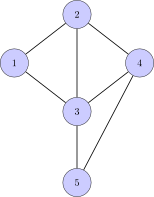
\includegraphics{bygraf.svg}

This network has a so called $5\times 5$ \emph{incidence matrix}, where city $i$ is associated with the
$i$-th row and $i$-th column. A $1$ in the matrix in the $(i, j)$ entry means that there is a road
from city $i$ to city $j$, whereas a $0$ means that city $i$ and city $j$ are not connected by a road:
$$
A = \begin{pmatrix}
0 & 1 & 1 & 0 & 0\\
1 & 0 & 1 & 1 & 0\\
1 & 1 & 0 & 1 & 1\\
0 & 1 & 1 & 0 & 1\\
0 & 0 & 1 & 1 & 0
\end{pmatrix}.
$$
Here
$$
A^2 =  
\begin{pmatrix}
2 & 1 & 1 & 2 & 1 \\
1 & 3 & 2 & 1 & 2 \\
1 & 2 & 4 & 2 & 1 \\
2 & 1 & 2 & 3 & 1 \\
1 & 2 & 1 & 1 & 2 
\end{pmatrix}\quad\text{and}\quad
A^3 =
\begin{pmatrix}
 2 & 5 & 6 & 3 & 3 \\
 5 & 4 & 7 & 7 & 3 \\
 6 & 7 & 6 & 7 & 6 \\
 3 & 7 & 7 & 4 & 5 \\
 3 & 3 & 6 & 5 & 2 
\end{pmatrix}.
$$
What is the interpretation of $A^2, A^3$ and  $A^n$ in general?
It turns out that the entry $(i, j)$ in the matrix $A^n$ exactly is
the number of paths of length $n$ from city $i$ to city $j$.


For example, there are $3$ paths from city $1$ to city $5$ of length $3$
corresponding to the paths $1245, 1345, 1235$.  The $2$ paths from city $1$ to city $1$ of
length $3$ are $1231, 1321$ and the  $5$ paths of length $3$ from city $1$ to city 
$2$ are $1342, 1242, 1312, 1212, 1232$.


\begin{hideinbutton}{A deeper explanation}
Suppose that we have a network with $m$ cities and incidence matrix $A$.

The general proof of the observations above in our special example, builds on the
fact that 
a path of length $n$ from city $i$ to city $j$ has to end with a road from a neighboring city
$k$ to $j$.
For every one of these neighboring cities, we may count the number of paths of length $n-1$
from city $i$.
If $A^{n-1}_{gh}$ is the number of paths of length $n-1$ from city $g$ to city $h$,
then matrix multiplication tells us that 
$$
A^n_{i j} = A^{n-1}_{i 1} A_{1 j} + \cdots + A^{n-1}_{i m} A_{m j} 
$$
This number is exactly the number of paths of length $n$ from city $i$ to
city $j$, since 
$A_{k j} = 1$ only when $k$ is a neighboring city to city $j$ (and $0$ otherwise).
\end{hideinbutton}
\end{example}

\section{Matrix arithmetic}\index{matrix arithmetic}

Matrix multiplication is very different from ordinary multiplication of numbers:
it is not \url{commutative}{https://en.wikipedia.org/wiki/Commutative_property}.
Consider the matrices
$$
A=
\begin{pmatrix}
0 & 1\\
0 & 0
\end{pmatrix}\qquad\text{and}\qquad
B = 
\begin{pmatrix}
0 & 0\\
1 & 0
\end{pmatrix}.
$$
Then
$$
A B = \begin{pmatrix} 1 & 0 \\ 0 & 0\end{pmatrix}\qquad \text{and} \qquad 
B A = \begin{pmatrix} 0 & 0 \\ 0 & 1\end{pmatrix}
$$
i.e.., $A B \neq B A$. 

\begin{sage}
import numpy as np
  
A = np.matrix( [[1, 1], [0, 1]] )
B = np.matrix( [[1, 0], [1, 1]] )
print("A =")
print(A)
print("B =")
print(B)
print("AB=")
print(A*B)
print("BA=")
print(B*A)
\end{sage}



Addition of matrices is like ordinary addition, except that you add all the entries of
the involved matrices.

\subsection{Matrix addition}\index{addition of matrices}

Addition of two matrices with the same number of rows and columns is defined below.
$$
\begin{pmatrix}
a_{11} & \cdots & a_{1 n} \\
\vdots & \ddots & \vdots\\
a_{m1} & \cdots & a_{m n}
\end{pmatrix} +
\begin{pmatrix}
b_{11} & \cdots& b_{1 n} \\
\vdots & \ddots & \vdots\\
b_{m1} & \cdots & b_{m n}
\end{pmatrix}
=
\begin{pmatrix}
a_{11} + b_{11} & \cdots & a_{1 n} + b_{1n}\\
\vdots & \ddots  & \vdots\\
a_{m1}+b_{m1} & \cdots & a_{m n}+b_{mn}
\end{pmatrix}.
$$

The zero matrix is the ($m\times n$) matrix containing zero in all its entries. When its number of
rows and columns are clear from the context it is simply denoted by $0$. For $2\times 3$ matrices
for example, we write
$$
0 =
\begin{pmatrix}
  0 & 0 & 0\\
  0 & 0 & 0
\end{pmatrix}.
$$


\beginshex
  Given an example of a non-zero $2\times 2$ matrix, such that
  $$
  A^2 = 0.
  $$
\endshex

\subsection{Multiplication of a number and a matrix}\index{multiplication of matrix med number}

A matrix may be multiplied by a number $\lambda$ by multiplying each entry by the number:
$$
\lambda \begin{pmatrix}
a_{11} & \cdots & a_{1 n} \\
\vdots & \ddots & \vdots\\
a_{m1} & \cdots & a_{m n}
\end{pmatrix} =
\begin{pmatrix}
\lambda a_{11} & \cdots & \lambda a_{1 n} \\
\vdots & \ddots & \vdots\\
\lambda a_{m1} & \cdots & \lambda a_{m n}
\end{pmatrix}.
$$

\beginshex
Does there exists a number  $\lambda$, such that 
$$
\lambda 
\begin{pmatrix}
1 & 2 & 3\\
4 & 5 & 6
\end{pmatrix} 
+
\begin{pmatrix}
0 & 0 & 0\\
0 & 0 & 2
\end{pmatrix} 
= 
\begin{pmatrix}
2 & 4 & 6\\
8 & 10 & 15
\end{pmatrix}?
$$
\endshex


\beginshex
Let $A$ be a $2\times 2$ matrix, such that
$$
A B = B A,
$$
for every other $2\times 2$ matrix $B$. Show that $A$ is a diagonal matrix of the form
$$
A =
\begin{pmatrix}
  a & 0\\
  0 & a
\end{pmatrix},
$$
where $a\in \RR$ i.e., $A = a I_2$.
\endshex


\subsection{The distributive law}

Ordinary numbers $a, b, c$ satisfy
$a (b + c) = a b + a c$. This rule also holds for
matrices and is called the distributive law (multiplication
is distributed over plus)

\begin{proposition}
Let $B$ and $C$ be $m\times n$ matrices, $A$ an $r\times m$ matrix and $D$ an $n\times s$ matrix. Then
$$
A ( B + C) = A B + A C\qquad\text{and}\qquad (B + C) D = B D + C D.
$$
\end{proposition}
\begin{proof}[showhide]
  Let us start by looking at $A(B+C) = A B + A C$. 
Here it suffices to do the proof, when $A$ is a row vector and
$B, C$ column vectors, since
$$
(A (B+C))_{ij} = A_i (B+C)^j = A_i (B^j + C^j).
$$
For $(B + C) D = B D + C D$, we may reduce to the case, where
$B, C$ are row vectors and  $D$ a column vector, since
$$
((B+C) D)_{ij} = (B+C)_i D^j = (B_i + C_i) D^j.
$$
Both of these cases follow using the distributive law for ordinary numbers.
\end{proof}




\beginshex
Suppose that $A$ and $B$ are two $2\times 2$ matrices. Is it true that
$$
(A + B)^2 = A^2 + B^2 + 2 A B?
$$
What about
$$
(A + B) (A - B) = A^2 - B^2?
$$
\endshex



\subsection{The miraculous associative law}

It does not make sense to multiply three matrices $A, B$ and $C$. We have only defined
matrix multiplication for two matrices. There are two natural ways of evaluating
$A B C$:
$$
( A B ) C\qquad \text{and}\qquad A (B C).
$$

We can begin by multiplying $A$ by $B$ and then multiply $C$ from the right.
However, we may just as well start by multiplying $B$ by $C$ and then
multiply $A$ from the left.

It is in no way clear, that these two computations give the same result!

That this turns out to be true, is just one of many miracles in the universe (there is a
rather cool mathematical explanation, though, addressed in an exercise below).

\begin{theorem}\label{thmmatmultass}
Let $A$ be an $m\times n$ matrix, $B$ an $n\times r$ matrix and $C$ an $r\times s$ matrix. Then
$$
(A B) C = A (B C).
$$
\end{theorem}
\begin{proof}[showhide]
  We must prove that 
$$
((A B) C)_{ij} = (A (B C))_{ij}
$$
for $1\leq i \leq m$ og $1\leq j \leq s$. The left hand side can be written
\begin{align}\label{eqleft}
(A B)_i C^j &= (A_i B^1, \dots, A_i B^r) C^j\\
            &= (A_i B^1) C_{1j} + (A_i B^2) C_{2j} + \cdots + (A_i B^r) C_{rj}.
\end{align}
The right hand side is 
\begin{equation}\label{eqright}
A_i (B C)^j = A_i \begin{pmatrix} B_1 C^j \\ \vdots \\ B_n C^j\end{pmatrix}
            = A_{i1} (B_1 C^j) + \cdots + A_{in} (B_n C^j).
          \end{equation}

          Writing the row-column multiplications in \eqref{eqleft}, we get
\begin{align}\label{rowscomp}
&A_{i1} B_{11} C_{1j} + \cdots + A_{in} B_{n1} C_{1j} +\\
&A_{i1} B_{12} C_{2j} + \cdots + A_{in} B_{n2} C_{2j} +\\
&\vdots\\
&A_{i1} B_{1r} C_{rj} + \cdots + A_{in} B_{nr} C_{rj}.
\end{align}
          Writing the row-column multiplications in \eqref{eqright}, we get
\begin{align}\label{colscomp}
&A_{i1} B_{11} C_{1j} + \cdots + A_{i1} B_{1r} C_{rj} +\\
&A_{i2} B_{21} C_{1j} + \cdots + A_{i2} B_{2r} C_{rj} +\\
&\vdots\\
&A_{in} B_{n1} C_{1j} + \cdots + A_{in} B_{nr} C_{rj}.
\end{align}
The rows in the sum in  \eqref{rowscomp} correspond to the columns in the sum \eqref{colscomp}.
Therefore these sums are equal and $((A B) C)_{ij} = (A (B C))_{ij}$.
\end{proof}

\begin{frameit}
\begin{remark}
The associative law $(A B) C = A (B C)$ is true, but in computing $A B C$ there can be a (big)
difference in the number of multiplications in the two computations
$A (B C)$ and $(A B) C$ i.e., efficiency is not associative for
matrix multiplication. In the notation of Theorem \ref{thmmatmultass}, computing
$(A B) C$ requires
$$
m n r + m r s = m r (n + s)
$$
multiplications, whereas computing $A (B C)$ requires
$$
n r s  + m n s = n s (m + r)
$$
multiplications. If for example $m=10000, n = 10, r = 10000$ and $s = 10$, then computing
$(A B) C$ requires $2\cdot 10^9$ multiplications, whereas
computing $A (B C)$ requires $2\cdot 10^6$ multiplications!   
\end{remark}
\end{frameit}


\beginshex
Verify the associative law for the three matrices
$$
A =
\begin{pmatrix}
  1 & 2\\
  3 & 4
\end{pmatrix}, \qquad
B =
\begin{pmatrix}
  1 & 2 & 3\\
  4 & 5 & 6
\end{pmatrix}\qquad\text{and}\qquad
C =
\begin{pmatrix}
  6 & 3\\
  5 & 2\\
  4 & 1
\end{pmatrix}
$$
by showing by explicit computation that
$$
(A B) C = A (B C).
$$
\endshex

\beginshex
There is in fact a high tech explanation that the associative law for matrices holds. An explanation
that makes the calculations in the above proof superfluous and shows the raw power of
abstract mathematics: suppose that
$f: \RR^n\rightarrow \RR^m, g:\RR^r\rightarrow \RR^n$ and $h:\RR^s\rightarrow \RR^r$ are linear maps.
Then $f\circ (g\circ h)$ and $(f\circ g)\circ h$ are both linear maps from $\RR^s\rightarrow \RR^m$, such that
$$
(f\circ (g\circ h))(x) = ((f\circ g)\circ h)(x) = f( g ( h (x)))
$$
for every $x\in \RR^s$. How does this relate to the associative law for matrix
multiplication?
\endshex

\section{The inverse matrix}

You are allowed to divide by a number provided it is $\neq 0$. Does it makes sense
to divide by matrices?

It does, but there are some matrices that correspond to the number $0$ that we are not allowed
to divide by.

\beginshex
Let $A, B$ and $C$ be $n\times n$ matrices. Show that
$$
B A = I_n
$$
and
$$
A C = I_n
$$
implies that $B = C$.
\endshex

\index{invertible matrix}\index{inverse matrix}

\begin{definition}
An $n\times n$ matrix $A$ is called invertible, if there exists an  $n\times n$ matrix $B$, such that 
$$
A B = B A = I_n.
$$
In this case, $B$ is called the inverse matrix of $A$ and denoted $A^{-1}$.
\end{definition}



\beginshex
Show that a quadratic matrix with a column or row consisting entirely of zeros cannot
be invertible.
\endshex

\beginshex
Suppose that
$$
A = \begin{pmatrix}
  a & b\\
  c & d
  \end{pmatrix}
  $$
  with $D = a d - b c\neq 0$. Prove that $A$ is invertible with
  $$
  A^{-1} = \frac{1}{D}\begin{pmatrix} d & -b\\ -c & a \end{pmatrix}.
  $$
\endshex


\beginshex
When is a quadratic diagonal matrix invertible? Look first at the $2\times 2$ case:
$$
\begin{pmatrix}
  a & 0\\
  0 & d
\end{pmatrix}.
$$
\endshex

The inverse matrix can be computed in \texttt{numpy}:

\begin{sage}
import numpy as np

A = np.matrix( [[5, 3], [3, 2]] )
print("The inverse of")
print(A)
print("is")
print(A.I)

\end{sage}

The inverse matrix enters the picture when solving $n$ linear
equations with $n$ unknowns:
\begin{align*}
a_{11}x_1 + a_{12} x_2 + \cdots + a_{1n} x_n &= b_1\\
&\vdots\\
a_{n1} x_1 + a_{n2} x_2 + \cdots + a_{nn} x_n &= b_n
\end{align*}
can be rewritten using matrix notation as 
$$
\begin{pmatrix}
a_{11} &  \cdots & a_{1 n} \\
\vdots & \ddots & \vdots\\
a_{n1} & \cdots & a_{n n}
\end{pmatrix}
\begin{pmatrix}
x_1 \\ \vdots \\ x_n
\end{pmatrix}
= 
\begin{pmatrix}
b_1 \\ \vdots \\ b_n
\end{pmatrix}
$$
or more compactly as $A x = b$.



If $A$ is invertible, then the associative law gives the following:
\label{ainvsol}
\begin{frameit}
\begin{align*}
A x &= b \iff\\
 A^{-1}  \left(A x\right) &= A^{-1} b \iff \\
(A^{-1} A) x &= A^{-1} b \iff\\
I x &= A^{-1} b\iff\\
x &= A^{-1} b.\\ 
\end{align*}
\end{frameit}

The inverse matrix gives the solution to the linear equations $A x = b$ just by one matrix multiplication!

\begin{example}
  The system of linear equations
\begin{equation}\label{simplign}
\begin{matrix}
&5 x &+ &3 y &= &13\\
&3 x &+&2 y &= &8
\end{matrix}
\end{equation}
can be rewritten using matrix multiplication to
$$
A v = b,
$$
where
$$
A = \begin{pmatrix}
5& 3 \\ 
3 & 2
\end{pmatrix}, \qquad
v = 
\begin{pmatrix} x \\ y \end{pmatrix}\qquad \text{and}\qquad
b = \begin{pmatrix} 13 \\ 8 \end{pmatrix}.
$$ 

Here $A$ is invertible and
$$
A^{-1} = 
\begin{pmatrix}
2 & -3\\
-3 & 5
\end{pmatrix}.
$$
One simple matrix multiplication
$$
\begin{pmatrix} x \\ y \end{pmatrix} = 
\begin{pmatrix}
2 & -3\\
-3 & 5
\end{pmatrix} \begin{pmatrix} 13 \\ 8 \end{pmatrix} = 
\begin{pmatrix} 2 \\ 1 \end{pmatrix}
$$
shows the solution we expect from  \eqref{simplign}.
\end{example}


The product of two invertible matrices (when this makes sense)
is an invertible matrix. This is the content of the following result.

\label{prodinv}
\begin{proposition}
The product $A B$ of  two invertible matrices $A$ and $B$ is invertible and
$(A B)^{-1} = B^{-1} A^{-1}$.
\end{proposition}
\begin{proof}[showhide]
We must check that 
$$
(B^{-1} A^{-1}) (A B) = I\qquad\text{and}\qquad A B (B^{-1} A^{-1}) = I.
$$
Let us check the first condition using the associative law:
\begin{align*}
(B^{-1} A^{-1}) (A B) &= ((B^{-1} A^{-1}) A) B\\
                    &= (B^{-1} (A^{-1} A)) B \\
                    &= (B^{-1} I) B = B^{-1} (I B) = B^{-1} B = I,
\end{align*}
where  $I$ denotes the identity matrix. The condition $A B (B^{-1} A^{-1}) = I$ is verified in the
same way.
\end{proof}


\beginshex

  We have defined a matrix $A$ to be invertible if there exists a matrix $B$, such that
  $A B = I$ and $B A = I$. Suppose that only $B A = I$. Can we then conclude that $A B = I$?

\endshex


\beginshex
Let
$$
N =
\begin{pmatrix}
  0 & 1 & 1 & 1\\
  0 & 0 & 1 & 1\\
  0 & 0 & 0 & 1\\
  0 & 0 & 0 & 0
\end{pmatrix}.
$$
Compute the powers $N^k$ for $k\geq 2$ i.e., $N^2, N^3, \dots$. Now let
$$
A = I + N,
$$
where $I = I_4$.
Show that $A$ is invertible, and
$$
A^{-1} = I - N + N^2 - N^3.
$$
Compute $A^{-1}$.

Do you see a way of generalizing this computation to 
$n\times n$ matrices $N$ with a property shared by the
$4\times 4$ matrix above?

\endshex

\subsection{Well, how do I find the inverse of a matrix?}

Finding the inverse of a matrix or deciding that the matrix is not invertible is
a matter of solving systems of linear equations.

Given an $n\times n$ matrix $A$, we need to see if there exists an $n\times n$ matrix
$B$, such that
\begin{equation}\label{invdef}
A B = I,
\end{equation}
where $I = I_n$ is the identity matrix of order $n$. We can do this by
computing the columns of $B$. From the definition in \eqref{invdef}, the
$j$-th column $B^j$ of $B$ must satisfy
\begin{equation}\label{lineqinv}
A B^j = I^j.
\end{equation}
This follows from the definition of matrix multiplication!

The identity in \eqref{lineqinv} is a system of $n$ linear equations
in $n$ unknowns. The unknowns are the entries in the $j$-th column
$B^j$ of the inverse matrix $A^{-1}$ (if it exists).

\begin{example}\label{exinverse}
  Suppose that $A$ is a $2\times 2$ matrix. Then the inverse matrix
  $B$ (if it exists) can be computed from the systems of linear
  equations below.
  $$
  A B^1 = \begin{pmatrix} 1 \\ 0 \end{pmatrix}\qquad\text{and}\qquad A B^2 = \begin{pmatrix} 0 \\ 1 \end{pmatrix}.
  $$
  Writing
  $$
  \begin{pmatrix} x \\ y \end{pmatrix} = B^1\qquad\text{and}\qquad \begin{pmatrix} u \\ v\end{pmatrix} = B^2
  $$
  for the first and second columns, the systems of linear equations can be written as
$$
\begin{matrix}
  &A_{11} x &+  &A_{12} y &=  &1\\
  &A_{21} x &+  &A_{22} y &=  &0
\end{matrix}\qquad\text{and}\qquad
\begin{matrix}
  &A_{11} u &+  &A_{12} v &=  &0\\
  &A_{21} u &+  &A_{22} v &=  &1
\end{matrix},
$$
where
$$
B =
\begin{pmatrix}
  x & u\\
  y & v
\end{pmatrix}.
$$
A concrete example along with a useful way of keeping track of the computation is presented in the video below.

\begin{video}
\youtube{4BX3eW4qo3g}
\end{video}
\end{example}

\beginshex
Compute the inverse of the matrix
$$
A =
\begin{pmatrix}
  1 & 1 & 1\\
  1 & 2 & 1\\
  1 & 1 & 3
\end{pmatrix}
$$
by employing the method of solving linear equations above. Explain
the steps in your computation. You may find it useful to collect
inspiration from the video in Example \ref{exinverse}.
\endshex

\section{The transposed matrix}\index{transposed matrix}

The transpose of an $m\times n$ matrix $A$ is the $n\times m$ matrix $A^T$ given by
$$
A^T_{i j} = A_{j i}.
$$
As an example, we have
$$
\begin{pmatrix}
0 & 2 & 4 & -2\\
3 & 2 & 7 & 4
\end{pmatrix}^T =
\begin{pmatrix}
0 & 3\\
2 & 2\\
4 & 7\\
-2 & 4
\end{pmatrix}.
$$
Notice also that $(A^T)^T = A$ for an arbitrary matrix $A$.

\begin{proposition}\label{prop:transformel}
Let $A$ be an $m\times r$ matrix and $B$ an $r\times n$ matrix. Then
$$
(A B)^T = B^T A^T.
$$
\end{proposition}
\begin{proof}[showhide]
  By definition $(A B)^T_{i j} = (A B)_{j i}$. This entry is given
  by row-column multiplication of the $j$-th row in $A$ and 
the $i$-th column in  $B$, which is the row-column multiplication of the
$i$-th row  in $B^T$ and the $j$-th column  in $A^T$.
\end{proof}

\beginshex
Let $A$ be a quadratic matrix. Prove that $A$ is invertible if and only if
$A^T$ is invertible.
\endshex

\beginshex In the sage window below, you are supposed to experiment a
bit by entering an arbitrary matrix $B$ and studying the quadratic
matrix $B B^T$. Is there anything special about this product?  Press
the \emph{Further explanation} button below the sage window to display
the rest of the exercise after(!) you have completed your
experimentation.

\begin{sage}
import numpy as np

B = np.matrix( [[1, 2, 3], [4, 5, 6], [7, 8, 9]] )
print("B is ")
print(B)
print("B times the transpose of B is ")
print(B*np.transpose(B))
\end{sage}

\begin{hideinbutton}{Further explanation}
  A quadratic matrix $A$ is called symmetric if $A = A^T$. Prove that
$$
B B^T
$$
is a symmetric matrix, where $B$ is an arbitrary matrix.
\end{hideinbutton}
\endshex

\section{Symmetric matrices}\label{Sectionsymmat}

A (quadratic) matrix $A$ is called symmetric if $A = A^T$. Visually,
this means that $A$ is symmetric around the diagonal like the
$3\times 3$ matrix
$$
\begin{pmatrix}
  1 & \cblue{2} & 3\\
  \cblue{2} & 5 & 4\\
  3 & 4 & 6
\end{pmatrix},
$$
but not like the $3\times 3$ matrix
$$
\begin{pmatrix}
  1 & \cblue{2} & 3\\
  \cred{4} & 5 & 6\\
  7 & 8 & 9
\end{pmatrix}.
$$

\beginshex
Show that
$$
B^T A B
$$
is a symmetric matrix, when $A$ is a symmetric matrix and
$B$ is an arbitrary matrix. Both matrices are assumed
quadratic of the same dimensions.
\endshex


If $A$ is a symmetric $n\times n$ matrix, we define the
function $f_A: \RR^n\rightarrow \RR$ given by
$$
f_A(v) = v^T A v.
$$

This definition is rather compact. You are encouraged to see the video below
for a specific example, when $A$ is a $2\times 2$ matrix.


\begin{video}\label{videoposdef}
  \youtube{YNwrLMJ8byM}
\end{video}




Inside set of the symmetric matrices we find two very important subsets
of matrices: the positive definite and the positive semi-definite
matrices. They correspond to positive and non-negative
real numbers.

\subsection{Positive definite matrices}

A symmetric matrix $A$ is called \emph{positive definite} if
$$
f_A(v) > 0
$$
for every $v\in \RR^n\setminus\{0\}$.

\beginshex
Give examples of (non-zero) $1\times 1$ and $2\times 2$ matrices that are
positive definite and ones that fail to be positive
definite.

When is a $2\times 2$ diagonal matrix positive definite?
\endshex

\beginshex
Let $A$ be a symmetric $n\times n$ matrix. Show that
$A$ is not positive definite if $A_{11} < 0$.
\endshex


\subsection{Positive semi-definite matrices}

A symmetric matrix $A$ is called \emph{positive semi-definite} if
$$
f_A(v) \geq 0
$$
for every $v\in \RR^n$.

From the definitions it follows that a positive definite matrix is
positive semi-definite.

\beginshex
Give an example of a non-zero matrix that is positive semi-definite,
but not positive definite.

When is a $2\times 2$ diagonal matrix positive semi-definite?
\endshex


\subsection{Symmetric reductions}

As you probably have noticed, it is rather straightforward to
see when a diagonal matrix is positive (semi)definite. For a
general symmetric matrix, one needs to transform to
an equivalent diagonal matrix. This is done
using the following result.

\begin{proposition}
  Let $A$ be a symmetric $n\times n$ matrix and $B$ an
  invertible $n\times n$ matrix. Then $A$ is
  positive (semi) definite if and only if
  $$
  B^T A B
  $$
  is positive (semi) definite.
\end{proposition}
  \begin{proof}[showhide]
    Every vector $v\in \RR^n$ is equal to $B u$ for a unique $u\in \RR^n$,
    since $B$ is invertible. Why? The upshot is that the equation
$$
v = B u
$$
can be solved by multiplying both sides by $B^{-1}$ giving
$$
v = B u \iff B^{-1} v = B^{-1} (B u) = (B^{-1} B) u = u.
$$



    So we get
    $$
    v^T A v = (B u)^T A (B u) = u^T (B^T A B) u.
    $$
    This computation shows that $A$ is positive (semi) definite if
    $B^T A B$ is positive semi-definite. The same
    reasoning with $u = B^{-1} v$ shows that $B^T A B$ is
    positive (semi) definite if $A$ is positive (semi) definite.

    Notice that it is important that $B v = 0$ only happens
    when $v=0$.
  \end{proof}


\beginshex
Let
$$
D =
\begin{pmatrix}
  d & 0\\
  0 & e
\end{pmatrix}
$$
be a diagonal matrix. What conditions must the diagonal
entries $d$ and $e$ satisfy in order for
$D$ to be positive definite?

Let
$$
A =
\begin{pmatrix}
  a & c\\
  c & b
\end{pmatrix}
$$
denote a symmetric $2\times 2$ matrix, where $a\neq 0$. Let
$$
B =
\begin{pmatrix}
  1 & -\frac{c}{a}\\
  0 & 1
\end{pmatrix}.
$$
Show that $B$ is invertible and compute
$$
B^T A B.
$$
Use this to show that $A$ is positive definite if and only if
$a>0$ and $a b - c^2 > 0$.

Let $f:\RR^2\rightarrow \RR$ be the function defined by
$$
f(x, y) = 2 x^2 + 3 y^2 + 4 x y.
$$
Show that $f(x, y)\geq 0$ for every $x, y\in \RR$.
\endshex


\end{document}
